\chapter{Funzioni a due variabili}

\section{Insieme aperti e chiusi}

\begin{definition}[Insieme aperto]
Un insieme $A$ è aperto se per ogni $x \in A$ (ed un $r>0$) esiste l'intorno $B_r(x) \subseteq A$.
\end{definition}

\begin{example}[Insieme aperto]
$x^2+y^2<1$
\end{example}

\begin{definition}[Insieme chiuso]
Un insieme è chiuso se è il complementare di un insieme aperto.
\end{definition}

\begin{example}[Insieme chiuso]
$x^2+y^2>=1$
\end{example}

\section{Generalità}

\section{Limiti}

Diciamo che $\lim_{(x,y)\to(a,b)} f(x,y) = L$ se:
\begin{itemize}
\item ogni intorno di $(a,b)$ contenga altri punti del dominio di $f$, differenti da $(a,b)$
\item per ogni numero positivo $\epsilon$ esiste un numero positivo $\gamma(\epsilon)$ tale che $|f(x,y)-L|<\epsilon$ vale ogni volta che $(x,y)$ è nel dominio di $f$ e soddisfa $0<\sqrt{(x-a)^2+(y-b)^2}<\gamma$
\end{itemize}

\subsection{Proprietà dei limiti}
\begin{itemize}
\item Se il limite esiste, esso è unico.
\end{itemize}
\begin{figure}[H]
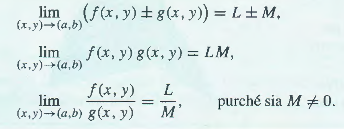
\includegraphics{prop-limiti.png}
\end{figure}
\section{Continuità}

Una funzione $f(x,y)$ si dice continua in un punto $(x_0,y_0)$ se:

\begin{itemize}
\item E' definita in $(x_0,y_0)$
\item Esiste il limite $\lim_{(x,y)\to(x_0,y_0)} f(x,y)$ ed è uguale a $f(x_0,y_0)$
\end{itemize}

Quindi non è detto che se esiste il limite di una funzione in un punto allora la funzione è definita in quel punto.

\section{Derivabilità}

\subsection{Derivata in $R$}

$$f'(x_0)=\lim_{h\to 0}\frac{f(x_0+h)-f(x_0)}{h}$$

\subsection{Derivate Parziali}

Calcolate solo rispetto all'asse $x$ o all'asse $y$.

\begin{figure}[H]
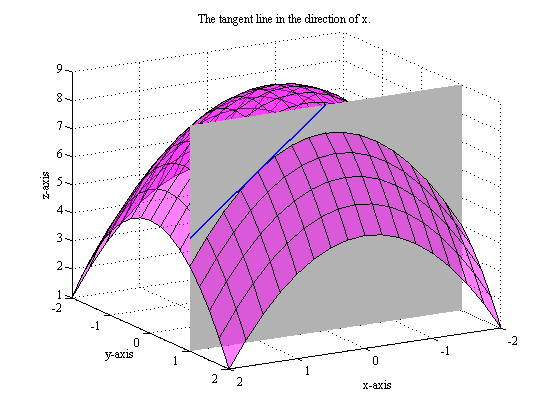
\includegraphics[width=\textwidth]{diff_partial.png}
\end{figure}

Limite di un quoziente di Newton rispetto a una delle due variabili.

$$
f_x(x_0,y_0) = \lim_{h\to 0} \frac{f(x_0+h,y_0)-f(x_0,y_0)}{h}
$$

$$
f_y(x_0,y_0) = \lim_{k\to 0} \frac{f(x_0,y_0+k)-f(x_0,y_0)}{k}
$$

\subsection{Derivata direzionale}

Ci forniscono la rapidità di variazione di $f(x,y)$ lungo una generica direzione $(a,b)$.

Calcolata rispetto ad una qualsiasi retta/direzione.

Fissato un qualunque vettore unitario $V=(v_1,v_2)$ posso calcolare:

$$
f_v(a,b) = \lim_{h\to 0_+} \frac{f(a+v_1h,b+v_2h)-f(a,b)}{h}
$$

La derivata direzionale è anche uguale a $$\nabla f(a,b)\cdot V$$

\subsection{Sviluppo di Taylor}

Rappresenta la migliore funzione polinomiale di grado $n$ che approssima la funzione $f$ in un intorno di $(x_0, y_0)$.

\begin{multline*}
f(x,y) = f(x_0,y_0)-f_x(x_0,y_0)(x-x_0)+f_y(x_0,y_0)(y-y_0)+ \\ \frac{1}{2} [f_{xx}(x_0,y_0)(x-x_0)^2+2f_{xy}(x_0,y_0)(x-x_0)(y-y_0)+f_{yy}(x_0,y_0)(y-y0)^2]+ \\ o((x-x_0)^2+(y-y_0)^2)
\end{multline*}

\section{Piano tangente}

\subsection{Vettore normale in un punto}

$$n = f_x(a,b)i+f_y(a,b)j-k$$

\subsection{Piano tangente}

Il piano tangente che passa per $P = (a,b,f(a,b))$ è $$f_x(a,b)(x-a)+f_y(a,b)(y-b)-(z-f(a,b))=0$$ cioè
$$z = f(a,b) + f_x(a,b)(x-a) + f_y(a,b)(y-b)$$

\section{Linearizzazione}

\subsection{In $R$}

La retta tangente al grafico $y=f(x)$ nel punto $x=a$ fornisce un' approssimazione dei valori di $f(x)$ per $x$ vicino ad $a$

$$f(x) \textasciitilde L(x) = f(a) + f'(a)(x-a)$$

\subsection{In $R^2$}

Il piano tangente al grafico di $z = f(x,y)$ in $(a,b)$ è $z = L(x,y)$ dove $$L(x,y) = f(a,b) + f_x(a,b)(x-a) + f_y(a,b)(y-b)$$ è la linearizzazione di $f(x,y)$ in $(a,b)$. La funzione $L(x,y)$ può essere usata per approssimare i valori di $f(x,y)$ vicino a $(a,b)$:
$$
f(x,y) \textasciitilde L(x,y) = f(a,b) + f_x(a,b)(x-a) + f_y(a,b)(y-b)
$$
\section{Differenziabilità}

\subsection{Differenziabilità in $R$}

Una funzione $f$ è differenziabile in $x_0$ se esiste un numero $\alpha \in R$ tale che:

$$f(x_0+h)=f(x_0)+\alpha h + o(h)$$

per $h \to 0$.

\subsection{Generalità}

Si dice che la funzione $f(x,y)$ è differenziabile in $(x_0,y0)$ se vale che:
$$
\lim_{(h,k)\to (0,0)} \frac{f(x_0+h,y_0+k) - f(x_0,y_0) - h A - k B}{\sqrt{h^2+k^2}} = 0
$$
dove $A=f_x(x_0,y_0)$ e $B=f_y(x_0,y_0)$

\subsection{Condizioni esistenza}

Per essere differenziabile una funzione deve essere continua e deve ammettere derivate parziali in $(a,b)$ lungo ogni direzione $V \in R^2$ (e quindi anche le derivate parziali).

Una funzione è differenziabile se e solo se la supericie $z=f(x,y)$ ha un piano tangente non verticale in $(a,b)$.

\section{Gradiente}

Chiamiamo $\nabla f(x_0,y_0)$ il gradiente della funzione $f$ calcolato in $(x_0,y_0)$.

$$ \nabla f(x_0,y_0) = (f_x(x_0,y_0),f_y(x_0,y_0))$$

Il vettore gradiente calcolato in un punto è anche detto \textbf{differenziale} della funzione in quel punto.

\subsection{Interpretazione geometrica}

\textbf{Per quali versori di $V$ la derivata direzionale risulta Massima o Minima?}

$$
f_V(x_0)  = |\nabla f(x_0)| \cdot |V| \cdot \cos(\theta)
$$

Visto che stiamo trattando versori allora $|V|=1$.

Quindi è la derivata direzionale è massima per $\cos(\theta)=1 \rightarrow \theta=0$

Quindi è la derivata direzionale è minima per $\cos(\theta)=0 \rightarrow \theta=\pi$

La direzione del gradiente calcolato in un punto indica la retta seguendo la quale si trova il massimo incremento della funzione $f$ nell'intorno del punto in cui è calcolato.

\subsection{Differenziale}

Se le derivate prime esistono, possiamo definire il differenziale: il differenziale di una funzione quantifica la variazione infinitesimale della funzione rispetto ad una variabile indipendente.

\section{Matrice Jacobiana}

La matrice jacobiana di una funzione è la matrice i cui elementi sono le derivate parziali prime della funzione.

La sua importanza è legata al fatto che, nel caso la funzione sia differenziabile, la jacobiana rappresenta la migliore approssimazione lineare della funzione vicino a un punto dato.

Sia $\mathbf{f}: U \rightarrow \mathbb R^m$ una funzione definita su un insieme aperto $U$ dello spazio euclideo  $\mathbb R^n$ . La matrice jacobiana della funzione $J {\mathbf f}$ in $\mathbf x = (x_1, \dots, x_n)$ è la matrice delle derivate parziali prime della funzione calcolate in $\mathbf x$:

$$J \, \mathbf f = \begin{bmatrix} \dfrac{\partial f_1}{\partial x_1} & \cdots & \dfrac{\partial f_1}{\partial x_n} \\ \vdots & \ddots & \vdots \\ \dfrac{\partial f_m}{\partial x_1} & \cdots & \dfrac{\partial f_m}{\partial x_n}  \end{bmatrix}\qquad \operatorname (J \, \mathbf f)_{ij} = \frac{\partial f_i (\mathbf {x})}{\partial x_j} $$

\section{Funzione omogenea}

\begin{definition}
Una funzione $f(x_1, \ldots, x_n)$ è detta positivamente omogenea di grado $k$ se, per ogni punto $(x_1, \ldots, x_n)$ del suo dominio e qualunque numero realte $t>0$ si ha
$$ f(tx_1, \ldots, tx_n) = t^k f(x_1, \ldots, x_n)$$

\subsection{Esempi}

$$f(x,y) = x^2 + xy - y^2$$
$$f(x,y) = \sqrt{x^2 + y^2}$$

\end{definition}

\section{Valori Estremi}

\subsection{Punti a cui prestare attenzione}

\begin{itemize}
\item Punti critici, $\nabla f(a,b) = 0$
\item Punti singolari, punti in cui $\nabla f(a,b) = 0$ non esiste
\item Punti di contorno del dominio di $f$
\end{itemize}

\subsection{Classificazione formale}

Se $(a,b)$ è punto critico allora guardo il segno di
$$\delta f = f(a+h,b+k)-f(a,b)$$

\subsection{Classificazione matrice hessiana}

$$
H(x,y) = \begin{vmatrix}
f_{xx} & f_{xy} \\
f_{xy} & f_{yy}
\end{vmatrix}
$$

\begin{itemize}
\item H(a,b) è definitia positiva, allora $f$ ha un minimo locale in $a$
\item H(a,b) è definitia negativa, allora $f$ ha un massimo locale in $a$
\item H(a,b) è indefinita, allora $f$ ha un punto di sella
\item H(a,b) = 0, allora questo test non ci dice nulla
\end{itemize}